\documentclass[11pt,]{article}
\usepackage[left=1in,top=1in,right=1in,bottom=1in]{geometry}
\newcommand*{\authorfont}{\fontfamily{phv}\selectfont}
\usepackage[]{mathpazo}


  \usepackage[T1]{fontenc}
  \usepackage[utf8]{inputenc}



\usepackage{abstract}
\renewcommand{\abstractname}{}    % clear the title
\renewcommand{\absnamepos}{empty} % originally center

\renewenvironment{abstract}
 {{%
    \setlength{\leftmargin}{0mm}
    \setlength{\rightmargin}{\leftmargin}%
  }%
  \relax}
 {\endlist}

\makeatletter
\def\@maketitle{%
  \newpage
%  \null
%  \vskip 2em%
%  \begin{center}%
  \let \footnote \thanks
    {\fontsize{18}{20}\selectfont\raggedright  \setlength{\parindent}{0pt} \@title \par}%
}
%\fi
\makeatother




\setcounter{secnumdepth}{3}

\usepackage{longtable,booktabs}

\usepackage{graphicx,grffile}
\makeatletter
\def\maxwidth{\ifdim\Gin@nat@width>\linewidth\linewidth\else\Gin@nat@width\fi}
\def\maxheight{\ifdim\Gin@nat@height>\textheight\textheight\else\Gin@nat@height\fi}
\makeatother
% Scale images if necessary, so that they will not overflow the page
% margins by default, and it is still possible to overwrite the defaults
% using explicit options in \includegraphics[width, height, ...]{}
\setkeys{Gin}{width=\maxwidth,height=\maxheight,keepaspectratio}

\title{Distribución y abundancia relativa de la familia Rubiaceae en la parcela
permanente Isla Barro Colorado\\
Subtítulo\\
Subtítulo  }



\author{\Large J. Alberto Meléndez Juan\vspace{0.05in} \newline\normalsize\emph{Universidad Autónoma de Santo Domingo (UASD)}  }


\date{}

\usepackage{titlesec}

\titleformat*{\section}{\normalsize\bfseries}
\titleformat*{\subsection}{\normalsize\itshape}
\titleformat*{\subsubsection}{\normalsize\itshape}
\titleformat*{\paragraph}{\normalsize\itshape}
\titleformat*{\subparagraph}{\normalsize\itshape}

\titlespacing{\section}
{0pt}{36pt}{0pt}
\titlespacing{\subsection}
{0pt}{36pt}{0pt}
\titlespacing{\subsubsection}
{0pt}{36pt}{0pt}





\newtheorem{hypothesis}{Hypothesis}
\usepackage{setspace}

\makeatletter
\@ifpackageloaded{hyperref}{}{%
\ifxetex
  \PassOptionsToPackage{hyphens}{url}\usepackage[setpagesize=false, % page size defined by xetex
              unicode=false, % unicode breaks when used with xetex
              xetex]{hyperref}
\else
  \PassOptionsToPackage{hyphens}{url}\usepackage[unicode=true]{hyperref}
\fi
}

\@ifpackageloaded{color}{
    \PassOptionsToPackage{usenames,dvipsnames}{color}
}{%
    \usepackage[usenames,dvipsnames]{color}
}
\makeatother
\hypersetup{breaklinks=true,
            bookmarks=true,
            pdfauthor={J. Alberto Meléndez Juan (Universidad Autónoma de Santo Domingo (UASD))},
             pdfkeywords = {palabra clave 1, palabra clave 2},  
            pdftitle={Distribución y abundancia relativa de la familia Rubiaceae en la parcela
permanente Isla Barro Colorado\\
Subtítulo\\
Subtítulo},
            colorlinks=true,
            citecolor=blue,
            urlcolor=blue,
            linkcolor=magenta,
            pdfborder={0 0 0}}
\urlstyle{same}  % don't use monospace font for urls

% set default figure placement to htbp
\makeatletter
\def\fps@figure{htbp}
\makeatother

\usepackage{pdflscape} \newcommand{\blandscape}{\begin{landscape}}
\newcommand{\elandscape}{\end{landscape}}


% add tightlist ----------
\providecommand{\tightlist}{%
\setlength{\itemsep}{0pt}\setlength{\parskip}{0pt}}

\begin{document}
	
% \pagenumbering{arabic}% resets `page` counter to 1 
%
% \maketitle

{% \usefont{T1}{pnc}{m}{n}
\setlength{\parindent}{0pt}
\thispagestyle{plain}
{\fontsize{18}{20}\selectfont\raggedright 
\maketitle  % title \par  

}

{
   \vskip 13.5pt\relax \normalsize\fontsize{11}{12} 
\textbf{\authorfont J. Alberto Meléndez Juan} \hskip 15pt \emph{\small Universidad Autónoma de Santo Domingo (UASD)}   

}

}








\begin{abstract}

    \hbox{\vrule height .2pt width 39.14pc}

    \vskip 8.5pt % \small 

\noindent Resumen del manuscrito


\vskip 8.5pt \noindent \emph{Keywords}: palabra clave 1, palabra clave 2 \par

    \hbox{\vrule height .2pt width 39.14pc}



\end{abstract}


\vskip 6.5pt


\noindent  \section{Introducción}\label{introducciuxf3n}

Las comunidades vegetales de los bosques neotropicales ejemplifican la
diversidad y complejidad ecológica de la región tropical. El estudio
continuo de la riqueza y la abundancia relativa en estas comunidades
permite identificar las especies raras, las cuales son más vulnerables a
los cambios en su hábitat y propensas a extinguirse localmente (Volkov,
Banavar, Hubbell, \& Maritan, 2003). Conocer estos aspectos de las
comunidades ecológicas y como se encuentran distribuidas en el espacio
las especies que las componen, ofrece la oportunidad de comprender como
evolucionan en el tiempo y los factores que inciden en su conservación
(Moreno, 2001).

Conocer si existe relación entre la ocurrencia de las distintas especies
de rubiaceas Son las condiciones ambientales y propiedades del suelo
factores que determinan como se organizan las especies de plantas en la
comunidad. Los parámetros de riqueza y abundancia relativa indicarán el
aporte de la familia rubiaceae a la diversidad de la comunidad y su
estructura. Como varía la diversidad alpha con respecto a condiciones
ambientales medibles, como por ejemplo la ácidez del suelo. Muchas
especies dentro de la familia rubiaceae son acidofilas y son
consideradas acumuladoras de aluminio{[}{]}. Además estudios anteriores
de la diversidad beta de la zona, especificamente del bosque tropical
panameño, sugieren una tendencia a la disimilaridad en la composición de
las comunidades entre sí que aumenta con la distancia en la cual las
comunidades se encuentran separadas en el espacio. (comunidades
comparadas lejanas unas de otras son más diferentes en cuanto a su
composición floristica).

Como se estructuran las comunidades ecológicas refiere al número de
individuos de cada taxa que las componen(Ricotta, 2004), además de su
distribución en el espacio. Este número se encuentra sujeto a diversas
variables las cuales aún no se conocen del todo ni en qué grado inciden
en la estructura de la comunidad (Neda, Horvat, Tohati, Derzsi, \&
Balogh, 2008).

La familia Rubiaceae es un importante grupo de plantas vasculares de
distribución cosmopolita con una marcada diversidad en regiones
tropicales y subtropicales (Davis et al., 2009). Las rubieaceas son
especialmente diversas en el neotrópico y resulta un grupo idóneo para
estudios ecológicos con énfasis en la estructura de las comunidades de
la región. Este trabajo intenta cuestionar la relación entre abundancia
relativa y distribución de las especies entre un mismo taxón superior,
en este caso tratandose de la familia rubiaceae. El número de individuos
de las distintas especies del mismo nivel trófico

\section{Metodología}\label{metodologuxeda}

\ldots

\section{Resultados}\label{resultados}

Como indica la tabla \ref{tab:abun_sp}

\begin{longtable}[]{@{}lr@{}}
\caption{\label{tab:abun_sp}Abundancia por especie.}\tabularnewline
\toprule
Latin & n\tabularnewline
\midrule
\endfirsthead
\toprule
Latin & n\tabularnewline
\midrule
\endhead
Faramea occidentalis & 24989\tabularnewline
Alseis blackiana & 7928\tabularnewline
Psychotria horizontalis & 2453\tabularnewline
Coussarea curvigemmia & 2010\tabularnewline
Palicourea guianensis & 1118\tabularnewline
Randia armata & 937\tabularnewline
Psychotria marginata & 761\tabularnewline
Alibertia edulis & 417\tabularnewline
Pentagonia macrophylla & 306\tabularnewline
Guettarda foliacea & 252\tabularnewline
Hamelia axillaris & 128\tabularnewline
Macrocnemum roseum & 87\tabularnewline
Posoqueria latifolia & 73\tabularnewline
Psychotria limonensis & 70\tabularnewline
Genipa americana & 67\tabularnewline
Psychotria graciliflora & 65\tabularnewline
Psychotria grandis & 57\tabularnewline
Psychotria deflexa & 38\tabularnewline
Amaioua corymbosa & 19\tabularnewline
Psychotria chagrensis & 16\tabularnewline
Psychotria acuminata & 14\tabularnewline
Tocoyena pittieri & 8\tabularnewline
Psychotria racemosa & 7\tabularnewline
Psychotria cyanococca & 4\tabularnewline
Chimarrhis parviflora & 3\tabularnewline
Coutarea hexandra & 3\tabularnewline
Psychotria brachiata & 3\tabularnewline
Appunia seibertii & 2\tabularnewline
Borojoa panamensis & 1\tabularnewline
Psychotria hoffmannseggiana & 1\tabularnewline
Rosenbergiodendron formosum & 1\tabularnewline
\bottomrule
\end{longtable}

\begin{figure}
\centering
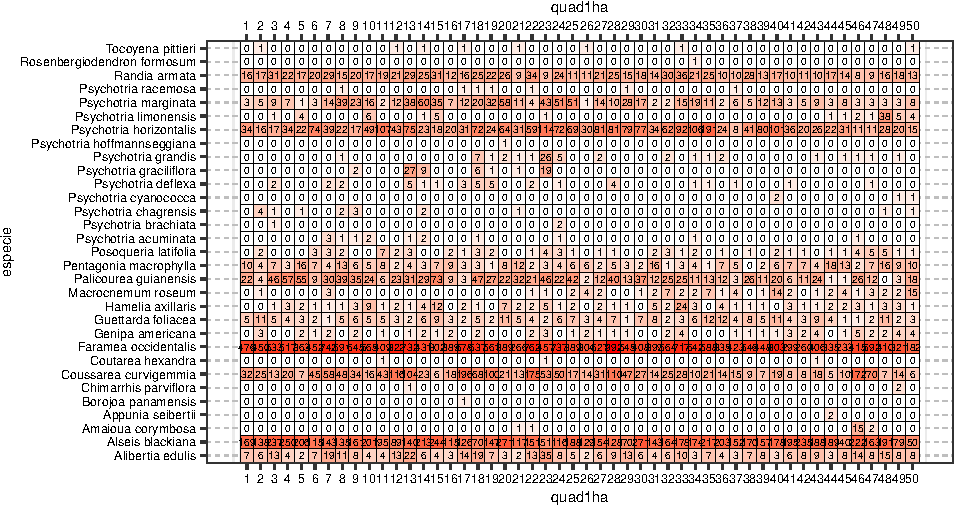
\includegraphics{manuscrito_files/figure-latex/unnamed-chunk-3-1.pdf}
\caption{\label{fig:abun_sp_q}Número de individuos de cada especie por
hectárea.}
\end{figure}

\begin{longtable}[]{@{}lllll@{}}
\toprule
c1 & c2 & c3 & c4 & c5\tabularnewline
\midrule
\endhead
adasdas & adasdadsadaadadadasdasdsau dadasdadadasdasdsaad & adasd & aasd
& asdsd\tabularnewline
adasddd & asadasdasd & adsadas & adad & asdasddad\tabularnewline
\bottomrule
\end{longtable}

\section{Discusión}\label{discusiuxf3n}

\section{Agradecimientos}\label{agradecimientos}

\section{Información de soporte}\label{informaciuxf3n-de-soporte}

\ldots

\section{\texorpdfstring{\emph{Script}
reproducible}{Script reproducible}}\label{script-reproducible}

\ldots

\section*{Referencias}\label{referencias}
\addcontentsline{toc}{section}{Referencias}

\hypertarget{refs}{}
\hypertarget{ref-davis2009global}{}
Davis, A. P., Govaerts, R., Bridson, D. M., Ruhsam, M., Moat, J., \&
Brummitt, N. A. (2009). A global assessment of distribution, diversity,
endemism, and taxonomic effort in the rubiaceae1. \emph{Annals of the
Missouri Botanical Garden}, \emph{96}(1), 68--78.

\hypertarget{ref-moreno2001manual}{}
Moreno, C. E. (2001). \emph{Manual de métodos para medir la
biodiversidad}. Universidad Veracruzana.

\hypertarget{ref-2008arXiv0803.3704N}{}
Neda, Z., Horvat, S., Tohati, H. M., Derzsi, A., \& Balogh, A. (2008). A
spatially explicit model for tropical tree diversity patterns.
\emph{arXiv E-Prints}, arXiv:0803.3704.

\hypertarget{ref-https:ux2fux2fdoi.orgux2f10.1111ux2fj.1366-9516.2004.00069.x}{}
Ricotta, C. (2004). A parametric diversity measure combining the
relative abundances and taxonomic distinctiveness of species.
\emph{Diversity and Distributions}, \emph{10}(2), 143--146.
\url{https://doi.org/https://doi.org/10.1111/j.1366-9516.2004.00069.x}

\hypertarget{ref-Volkov_2003}{}
Volkov, I., Banavar, J. R., Hubbell, S. P., \& Maritan, A. (2003).
Neutral theory and relative species abundance in ecology. \emph{Nature},
\emph{424}(6952), 1035--1037. \url{https://doi.org/10.1038/nature01883}




\newpage
\singlespacing 
\end{document}
